% File: leporello-doc.tex
% Copyright 2025 Jasper Habicht (mail(at)jasperhabicht.de).
%
% This work may be distributed and/or modified under the
% conditions of the LaTeX Project Public License version 1.3c,
% available at http://www.latex-project.org/lppl/.
%
% This file is part of the `leporello' package (The Work in LPPL)
% and all files in that bundle must be distributed together.
%
% This work has the LPPL maintenance status `maintained'.
%
\documentclass[a4paper]{article}
\def\leporellofileversion{1.0.2}
\def\leporellofiledate{10 September 2025}

\usepackage[T1]{fontenc}
\usepackage{Alegreya}
\usepackage{AlegreyaSans}
\usepackage{FiraMono}

\usepackage{geometry, longtable, booktabs, siunitx, tcolorbox, hyperref}
\geometry{margin=25mm, left=45mm}
\urlstyle{same}

\usepackage{fancyhdr}
\pagestyle{fancy}
\fancyhf{}
\renewcommand{\headrulewidth}{0pt}
\fancyfoot[R]{\thepage}

\ExplSyntaxOn
\NewDocumentCommand{\fnstars}{m}{
  \int_step_inline:nn { \value{#1} } { * }
}
\ExplSyntaxOff

\linespread{1.1}\selectfont
\addtolength{\skip\footins}{1em plus 5pt}
\makeatletter
\renewcommand*{\thefootnote}{\fnstars{footnote}}
\renewcommand{\@makefntext}[1]{%
  \noindent\hbox to 1em{\normalfont\@thefnmark\hss}~#1%
}
\makeatother

\tcbuselibrary{skins,listings}
\lstdefinestyle{leporellodocmacro}{
  basicstyle=\small\ttfamily,
  literate=*{<}{{{\color{black!50}\guilsinglleft}}}1
    {>}{{{\color{black!50}\guilsinglright}}}1,
  keywords={},
  moredelim=[is][\bfseries]{|}{|},
  moredelim=[is][\bfseries\itshape]{?}{?},
  moredelim=[is][\color{black!50}]{!}{!},
}
\lstdefinestyle{leporellodoccodeexample}{
  basicstyle=\small\ttfamily,
  keywords={},
}

\hypersetup{colorlinks}

\ExplSyntaxOn
\int_new:N \l_leporello_doc_change_int
\NewDocumentCommand{\changes}{ m m m }{
  \int_incr:N \l_leporello_doc_change_int
  \prop_new:c { l_leporello_doc_change_
    \int_to_roman:n { \l_leporello_doc_change_int } _prop }
  \prop_put:cnn { l_leporello_doc_change_
    \int_to_roman:n { \l_leporello_doc_change_int } _prop } { version } {#1}
  \prop_put:cnn { l_leporello_doc_change_
    \int_to_roman:n { \l_leporello_doc_change_int } _prop } { date } {#2}
  \prop_put:cnn { l_leporello_doc_change_
    \int_to_roman:n { \l_leporello_doc_change_int } _prop } { changes } {#3}
}
\NewDocumentCommand{\printchanges}{ }{
  \section{Changes}
  \begin{description}
    \setlength\itemsep{0pt}
    \int_step_inline:nn { \l_leporello_doc_change_int } {
      \item[
        \prop_item:cn { l_leporello_doc_change_
        \int_to_roman:n { ##1 } _prop } { version } ~
        \normalfont{ (
          \prop_item:cn { l_leporello_doc_change_
          \int_to_roman:n { ##1 } _prop } { date }
        ) }
      ]
      \prop_item:cn { l_leporello_doc_change_
      \int_to_roman:n { ##1 } _prop } { changes }
    }
  \end{description}
}

\tl_new:N \l_leporello_doc_doctitle_tl
\NewExpandableDocumentCommand{\makedoctitle}{ o m o m m o m }{
  \hypersetup{
    pdfauthor={#5},
    pdftitle={\IfValueTF{#1}{#1}{#2}},
    pdfsubject={\IfValueTF{#3}{#3}{#4}}
  }
  \tl_set:Nn \l_leporello_doc_doctitle_tl {
    \group_begin:
      \tcbset{
        title ~ style ~ hook/.style={
          boxrule=2pt,
          fontupper=\huge\ttfamily
        }
      }
      \setlength{\parindent}{0pt}\sffamily
      \Huge{\bfseries #2}\par\bigskip
      \Large #4\par\bigskip
      \large #5
      \IfValueT{#6}{
        \,\footnote{#6}\par\bigskip
      }
      #7\par\bigskip
      \rule{\textwidth}{.08em}
    \group_end:
  }
}

\NewExpandableDocumentCommand{\printdoctitle}{ }{
  \tl_use:N \l_leporello_doc_doctitle_tl
}
\ExplSyntaxOff

\NewDocumentCommand{\expandablestarcode}{ O{0,0} }{
  \fill[black!50, shift={([xshift={-10pt}, yshift={-10pt-0.5em}]#1)}]
    (90:3.75pt)
    \foreach \i in {1,...,4} {
      -- ({90+360/5*\i*2}:3.75pt)
    } -- cycle;
}

\NewDocumentCommand{\expandablestar}{}{
  \tikz{\expandablestarcode}
}

\NewDocumentCommand{\warning}{}{%
  \begin{tikzpicture}[overlay, baseline={(w.base)}]
    \node[circle, fill, black!25!red!10, text=black!25!red, outer sep=0pt]
      (w) at (-3em,0pt) {\bfseries !};
    \fill[black!25!red!10]
      (w.east) |- (w.south) -- cycle;
  \end{tikzpicture}%
}

\tcbset{
  size=small,
  arc=2.5pt,
  outer arc=2.5pt,
  colframe=black!10,
  colback=black!10,
  title style hook/.style={},
}

\NewTCBListing{macrodef}{ s o }{
  listing only,
  listing style={leporellodocmacro},
  grow to left by=2cm,
  boxrule=0pt,
  after={\par\smallskip\noindent},
  enhanced,
  IfValueT={#2}{
    hypertarget=#2
  },
  IfBooleanT={#1}{
    overlay={
      \expandablestarcode[frame.north east]
    }
  }
}

\NewTCBListing{codeexample}{ }{
  listing only,
  listing style={leporellodoccodeexample},
  after={\par\smallskip\noindent}
}

\NewTCBListing{codeexamplecolumns}{ }{
  text side listing,
  lefthand width=4.5cm,
  listing style={leporellodoccodeexample},
  after={\par\smallskip\noindent}
}

\NewTCBListing{macrodeprecated}{ s }{
  listing only,
  listing style={leporellodocmacro},
  boxrule=0pt,
  width={0.5\linewidth-2.5pt},
  box align=top,
  after=\hfill,
  colframe=black!25!red!10,
  colback=black!25!red!10,
  enhanced,
  IfBooleanT={#1}{
    overlay={
      \fill[black!25!red!10]
        ([yshift={5pt-1.5em}]frame.north east)
        -- ++(5pt,-5pt) -- ++(-5pt,-5pt)
        -- cycle;
    }
  }
}

\NewTCBListing{macroreplacement}{ }{
  listing only,
  listing style={leporellodocmacro},
  boxrule=0pt,
  width={0.5\linewidth-2.5pt},
  box align=top,
  before={},
  colframe=black!25!green!10,
  colback=black!25!green!10
}

\NewTotalTCBox{\macro}{ O{} v }{
  verbatim,
  size=tight,
  arc=1pt,
  outer arc=1pt,
  top=0.5pt,
  bottom=0.5pt,
  left=2pt,
  right=2pt,
  boxrule=0pt,
  colframe=black!10,
  colback=black!10,
  fontupper=\small\ttfamily,
  #1
}{\vphantom{/g}\lstinline^#2^}

\NewTotalTCBox{\titlemacro}{ s O{} m }{
  verbatim,
  size=tight,
  arc=1pt,
  outer arc=1pt,
  top=0.5pt,
  bottom=0.5pt,
  left=2pt,
  right=2pt,
  boxrule=0pt,
  colframe=black!10,
  colback=black!10,
  fontupper=\small\ttfamily,
  title style hook,
  #2
}{\vphantom{/g}\IfBooleanT{#1}{\textbackslash}#3}

\sisetup{detect-all}
\NewDocumentCommand{\mmdim}{m}{%
    \qty{#1}{\milli\metre}%
}

\makedoctitle
  [The leporello package]
  {The \titlemacro{leporello} class}
  {A simple LaTeX document class to create folded leaflets using columns and boxes}
  {Jasper Habicht}[E-mail: \href{mailto:mail@jasperhabicht.de}{mail@jasperhabicht.de}. Title image: \textcopyright{} 2025 Hannah Klöber.]
  {Version \leporellofileversion, released on \leporellofiledate}

\changes{v0.7.0}{2025/08/08}{First public beta release.}
\changes{v0.8.0}{2025/08/12}{Added box attachment mechanism and option to place arbitrary code to box background.}
\changes{v0.9.0}{2025/08/15}{Box attachment mechanism and flow mechanism use box name instead of ID. Enhanced pagination settings. Support for right-to-left and vertical typesetting.}
\changes{v0.9.2}{2025/08/18}{Various improvements and bug fixes.}
\changes{v0.9.3}{2025/08/22}{Stretch mechanism fixed.}
\changes{v0.9.5}{2025/08/25}{Improved alignment mechanism.}
\changes{v1.0.0}{2025/08/27}{Improved key management and flow mechanism. Added note mechanism.}
\changes{v1.0.1}{2025/08/30}{Fix of a bug that prevented the dimensions set with the keys \titlemacro{store width} and \titlemacro{store height} from having the correct value when used as value to the \titlemacro{offset} key. Fix of a bug in the stretch mechanism. Fix of a bug in right-to-left typesetting.}
\changes{v1.0.2}{2025/09/10}{Documented L3 commands.}

\begin{document}
\vspace*{-2.5em}
\noindent\hspace{-10pt}

\includegraphics[width=80mm]{doc/leporello.pdf}
\bigskip

\printdoctitle
\bigskip

\section{Introduction}

The \macro{leporello} class is a simple LaTeX document class to create folded leaflets with the following key features:

\begin{itemize}
  \item The document layout consists of a specific number of pages that can have varying widths and are placed next to each other. Each page contains one frame to contain typeset material.
  \item Material is typeset in boxes and boxes are positioned in columns which in turn are placed into the frames on the pages of the document.
  \item Columns are predefined and then placed into the frame of a page in the document layout. This way, columns can be used on pages with varying widths.
  \item Boxes can have padding (including bleed) and a background and are positioned inside a column.
\end{itemize}

A folded leaflet is sometimes called leporello in reference to the servant of Don Giovanni (known from the opera by Mozart) who, at one point, unfolds a lengthy zig-zag folded list of his master's love affairs.

There are some requirements for the creation of print data for high-quality folded leaflets: Especially if the leaflet is folded inward, the inner pages should be a bit less wide, so in general the pages of a leaflet are not of the exact same width (although the widths only differ slightly). Also, borderless printing requires that the print data adds a so-called bleed area added to the layout if the final document into which the typeset material extends. This area is trimmed off eventually to avoid unprinted edges due to natural movement of the paper during guillotining. Crop marks need to be added to the print data showing the layout of the final document. This packages takes into account all these requirements while providing a lot of customization.

\warning This document class is still in an early development phase which means that bugs cannot be ruled out and some things may not work properly. Also, updates may be published frequently. The author is grateful for reporting any bugs via GitHub at \url{https://github.com/jasperhabicht/leporello/issues}. A site for asking questions about the document class and for suggestions for improvement is available at \url{https://github.com/jasperhabicht/leporello/discussions}.

\section{Loading the document class}

Use \macro{\documentclass{leporello}} to load the document class. The document class loads the \macro{graphicx} and the \macro{l3draw} package.

The document class is based on the \macro{article} class to enable basic typesetting commands. But due to the redefinition of the layout, certain functions of the \macro{article} class, such as placing material into the header, the footer or the margin (which do not exist in the leporello layout) or using floats or footnotes won't work. Instead of floats, the document class provides a sophisticated alignment mechanism for boxes. Instead of footnotes, it provides its own note mechanism.

\begin{macrodef}
|\leporelloset|[<prefix>]{<options>}
\end{macrodef}
Use \macro{\leporelloset} or use the optional argument of the \macro{\documentclass} command to globally set the document layout. The optional argument can be used to set a common prefix to all options. Options should be used without the \macro{global/} prefix when used as option to the \macro{\documentclass} command. The following options are available:

\begin{macrodef}
global/|columns|={<list of dimensions>}
global/|two columns|
global/|three columns|
global/|four columns|
global/|four columns wrap|
global/|five columns|
global/|six columns|
\end{macrodef}
Expects a comma-separated list of dimensions that describe the widths of the columns in the layout. If \macro{columns} is not specified, the class assumes the default value of \macro{97mm, 100mm, 100mm}. The width of the document layout is automatically calculated from the dimensions set via \macro{columns}.

A few column layouts are predefined. These do not expect a value. The layouts will set the following list of dimensions:

\begin{longtable}{
  @{}
  p{\dimexpr0.35\linewidth-\tabcolsep}
  p{\dimexpr0.65\linewidth-\tabcolsep}
  @{}
}
  \toprule
  \textbf{Key}              & \textbf{List of dimensions}                                 \\
  \midrule
  \macro{two columns}       & \mmdim{99}, \mmdim{99}                                      \\
  \macro{three columns}     & \mmdim{97}, \mmdim{100}, \mmdim{100}                        \\
  \macro{four columns}      & \mmdim{99}, \mmdim{99}, \mmdim{99}, \mmdim{100}             \\
  \macro{four columns wrap} & \mmdim{97}, \mmdim{99}, \mmdim{100}, \mmdim{101}            \\
  \macro{five columns}      & \mmdim{97}, \mmdim{97}, \mmdim{97}, \mmdim{99}, \mmdim{100} \\
  \macro{six columns}       & \mmdim{99}, \mmdim{99}, \mmdim{96}, \mmdim{96}, \mmdim{100}, \mmdim{100} \\
  \bottomrule
\end{longtable}

\begin{macrodef}
global/|layout height|={<dimension>}
\end{macrodef}
Expects a dimension that sets the height of the final layout. If \macro{layout height} is not specified, the class assumes the default value of \macro{210mm} (the height of A4 landscape).

\begin{macrodef}
global/|auto typeset|
\end{macrodef}
If set, the columns are automatically typeset according to the order of the definition of the columns. This means that in a three-column layout for example, the first three defined columns will be placed on the first PDF page followed by the next three defined columns on the next PDF page. This key does not expect a value.

\begin{macrodef}
global/|show frames|
\end{macrodef}
If set, frames around the single pages (columns) are shown. This key does not expect a value.

\begin{macrodef}
global/|show ids|
\end{macrodef}
If set, the IDs of the boxes are shown. This key does not expect a value. The IDs of the boxes are integers starting from 1 and increasing in the order of typesetting of the boxes.

\begin{macrodef}
global/|prepress|
\end{macrodef}
If set, the paper size is increased at all four edges by the width of the info area and crop marks are placed at the corners. This key does not expect a value.

\begin{macrodef}
global/|info area|={<dimension>}
\end{macrodef}
Expects a dimension for the width of the info area that is shown if \macro{prepress} is set. If \macro{info area} is not specified, the class assumes the default value of \macro{10mm}.

\begin{macrodef}
global/|bleed|={<dimension>}
\end{macrodef}
Expects a dimension for the width of the bleed that is added to boxes with background and other material reaching to the edges of the document layout. If \macro{bleed} is not specified, the class assumes the default value of \macro{3mm}.

\begin{macrodef}
|\leporellobleed|
\end{macrodef}
Retrieves the width of the bleed in pt.

\begin{macrodef}
|\leporelloboxwidth|
\end{macrodef}
Retrieves the width of the current box including padding, but without bleed, in pt. The width of the box excluding padding can be retrieved with the \macro{\linewidth} command.

\section{Defining columns}

Columns are grouped material to be typeset onto a specific page of the folded leaflet. A column can contain anything that can be placed in a TeX box in general, but the typical use of a column is to only serve as a frame to which boxes are attached. While the package provides a flow mechanism across boxes, no such mechanism is provided for columns. Thus, if a column contains more than fits into it, the relevant parts just spill over the frame edges.

\begin{macrodef}
\null\begin{|leporellocolumn|}{<string>}
  <body>
\end{|leporellocolumn|}
\end{macrodef}
A column is defined by the \macro{leporellocolumn} environment which takes one mandatory argument taking the name of the column. A single dot (\macro{.}) is reserved as name for an empty column.

\section{Positioning boxes}

\begin{macrodef}
\null\begin{|leporellobox|}[<options>]
  <body>
\end{|leporellobox|}
\end{macrodef}
Boxes can be positioned inside of columns. They can contain anything that can be placed in a TeX box in general. A box is defined by the \macro{leporellobox} environment which takes one optional argument to set box-specific options. Options should be used without the \macro{box/} prefix when used as option to the \macro{leporellobox} environment. These are the following:

\begin{macrodef}
box/|name|={<string>}
\end{macrodef}
Expects a (unique) string denoting the name of the box which can be used for attaching boxes to one another or for assigning boxes for the flow mechanism. This key can only be set locally to the \macro{leporellobox} environment.

\begin{macrodef}
box/|parent|={<string>}
\end{macrodef}
Expects a string denoting the name of the box to which the current box is aligned. If not specified, the current column box is assumed as parent box. The parent box needs to be in the same column as the box that should be aligned to it. This key can only be set locally to the \macro{leporellobox} environment.

\begin{macrodef}
box/|align parent|={<tuple of poles>}
\end{macrodef}
Expects a comma-separated list of two items (a tuple) which denotes the horizontal and vertical pole of which the intersection defines the coordinate of the parent box (per default this is the current column box) that serves as anchor to align the current box. If not specified, the default value \macro{l, t} is assumed, denoting the top left corner. Available poles are:

\begin{longtable}{
  @{}
  p{3em}
  p{\dimexpr\linewidth-2\tabcolsep-3em}
  @{}
}
  \toprule
  \textbf{Key} & \textbf{Meaning}             \\*
  \midrule
  \macro{l}    & left edge of the box         \\
  \macro{hc}   & horizontal center of the box \\
  \macro{r}    & right edge of the box        \\
  \macro{t}    & top edge of the box          \\
  \macro{vc}   & vertical center of the box   \\
  \macro{b}    & bottom edge of the box       \\
  \bottomrule
\end{longtable}

\begin{macrodef}
box/|align self|={<tuple of poles>}
\end{macrodef}
Expects a comma-separated list of two items (a tuple) which denotes the horizontal and vertical pole of which the intersection defines the coordinate of the current box that serves as anchor to align the current box to parent box (per default this is the current column box). If not specified, the default value \macro{l, t} is assumed, denoting the top left corner. Available poles are the same as for \macro{align parent}.

\begin{macrodef}
box/|offset|={<tuple of dimensions>}
\end{macrodef}
Expects a comma-separated list of two dimensions (a tuple) which defines the offset of the anchor set via \macro{align parent} and \macro{align self}. The first dimension is the offset to the right, the second dimension the offset downwards. If not specified, the default value \macro{0mm, 0mm} is assumed. Internally, the value is parsed as a floating point variable.

\begin{macrodef}
box/|width|={<dimension>}
\end{macrodef}
Expects a dimension to explicitly set the width of the current box. If not specified, the box is as wide as the parent column.

\begin{macrodef}
box/|height|={<dimension>}
\end{macrodef}
Expects a dimension to explicitly set the height of the current box. If not specified, the box takes its natural height which means that it is as high as necessary to fit the contents.

\begin{macrodef}
box/|stretch|
\end{macrodef}
If set, the box is stretched until its relevant edge (the bottom edge if aligned at the top, the top edge if aligned at the bottom, in vertical typesetting the left or right edge) meets the edge of the parent column. This key does not expect a value.

This key can also help to align the relevant edges in cases where stretchable glue close to the edge would otherwise make the box overlap the edge of the parent column.

\begin{macrodef}
box/|padding left|={<dimension>}
box/|padding right|={<dimension>}
box/|padding top|={<dimension>}
box/|padding bottom|={<dimension>}
box/|padding|={<key-value list>}
box/|no padding|
\end{macrodef}
\macro{padding left}, \macro{padding right}, \macro{padding top} and \macro{padding bottom} each expect a dimension to describe the padding of the contents from the relevant edge of the box. If not specified, the default value of \macro{7.5mm} is assumed.

All four padding settings can also be stated using the \macro{padding} key and the subkeys \macro{left}, \macro{right}, \macro{top}, \macro{bottom}. Using this syntax, the default value of the padding setting would be expressed as \macro{padding={left=7.5mm, right=7.5mm, top=7.5mm, bottom=7.5mm}}.

The key \macro{no padding} sets all paddings to zero. This key does not expect a value.

\begin{macrodef}
box/|pre|={<code>}
\end{macrodef}
Expects a token list that is placed before the actual contents of the box. Should not contain typeset material. This can be handy, if multiple boxes should be styled in a similar way.

\begin{macrodef}
box/|background color|={<color name>}
box/|background color|={none}
\end{macrodef}
Expects a color name as defined via \macro{l3color} or \macro{none} which will not fill the background. If not specified, the default value of \macro{none} is assumed.

\begin{macrodef}
box/|background code|={<code>}
\end{macrodef}
Expects typeset material that will be placed into the background of the box aligned at the upper left corner of the box. THe typeset material is clipped to the size of the box.

\begin{macrodef}
box/|bleed|={<list of values>}
\end{macrodef}
Expects a comma-separated list consisting of up to four items with the values \macro{l} and \macro{r}, \macro{t} and \macro{b} that describe the edges (left, right, top and bottom) where bleed should be added to the box. Note that bleed is never added to the inner edges where the columns meet.

\begin{macrodef}
box/|store width|={<control sequence>}
\end{macrodef}
Expects a single control sequence (macro) to store the width of the current box.

\begin{macrodef}
box/|store height|={<control sequence>}
\end{macrodef}
Expects a single control sequence (macro) to store the height of the current box.

\begin{macrodef}
box/|flow into|={<string>}
\end{macrodef}
Expects a string denoting the name of the box into which typeset material will flow into if it does not fit into the current box. The box to flow into can be in a following column or on a following page. See section \ref{sec:flow} below. This key can only be set locally to the \macro{leporellobox} environment.

\section{Typesetting boxes into columns}

\begin{macrodef}
|\leporellotypesetcolumns|[<options>]{<list of strings>}
\end{macrodef}
Using the command \macro{\leporellotypesetcolumns} which takes one mandatory argument, previously defined columns can be placed onto a page of the document. The command expects as argument a comma-separated list of names of previously defined columns. These are then placed onto a document page from left to right while the width is taken from the setting via the \macro{columns} key and the height is taken from the setting via the \macro{layout height} key. With a \macro{.}, an empty column can be added to the list.

The command takes one optional argument. Options should be used without the \macro{typeset/} prefix when used as option to the \macro{\leporellotypesetcolumns} command. The command accepts the following options:

\begin{macrodef}
typeset/|reverse layout|
\end{macrodef}
If set, the widths of the columns are reversed, but the placement of the columns is still from left to right. This option does not take a value. The option should be used to typeset the verso of a folded leaflet that naturally has the widths of the columns reversed. This key does not expect a value.

\begin{macrodef}
typeset/|reverse order|
\end{macrodef}
If set, the order of the columns is reversed, which means that the columns are typeset from right to left. Pagination is not affected. This key does not expect a value.

\begin{macrodef}
typeset/|reverse pagination|
\end{macrodef}
If set, the pagination of the columns is reversed. This key does not expect a value.

\begin{macrodef}
typeset/|continuous pagination|
\end{macrodef}
If set, columns are numbered continuously from left to right. Otherwise, the pagination starts on the last column of every odd shipout page, continues from left to right over the columns on the following shipout page and eventually from left ro right over the remaining columns on the first page. For example, in a document with three columns per shipout page the pagination would be 5, 6, 1 and 2, 3, 4 and then on the next two shipout pages 11, 12, 7 and 8, 9, 10. This key does not expect a value.

\section{Flow mechanism}\label{sec:flow}

Typeset material can flow from one box to another box. To this end, the key \macro{flow into} can be set to the relevant box and assigned the name of the box to flow into as value. The name of the relevant box can be set via the \macro{name} key.

\begin{macrodef}
|\leporelloboxbreak|
\end{macrodef}
The flow mechanism works across multiple boxes. But due to the way the typesetting mechanism of TeX works, it needs some manual adjustment if the typeset material flows across boxes of different width. In this case, the command \macro{\leporelloboxbreak} or \macro{\pagebreak} should be inserted at the point where the break should take place. The command \macro{\leporelloboxbreak} is especially suited for justified typesetting as it will keep the last line before the break justified in contrast to the \macro{\pagebreak} command.

Typeset material can only flow into boxes in the following column or page. If typeset material should flow backwards on the same page, this can be achieved using the key \macro{reverse order} on the relevant page.

\subsection{Right-to-left and vertical typesetting}

The document class natively supports right-to-left and vertical typesetting using the mechanisms provided by LuaLaTeX. The \macro{babel} package also makes use of the mechanisms for bidirectional typesetting provided by LuaLaTeX, which means that this package will work best with a combination of LuaLaTeX and \macro{babel} for right-to-left or vertical typesetting.

If right-to-left typesetting is activated, the layout, order and pagination of the layout will be reversed automatically.

If the \macro{bidi} package is used (which is used by the \macro{polyglossia} package), the following addition to the preamble is needed to enable right-to-left typesetting:

\begin{codeexample}
\AddToHook{leporello/typeset/before}{\setLTR}
\AddToHook{leporello/box/begin}{\setRTL}
\end{codeexample}

In general, it has to be made sure that only the inner boxes are affected by the right-to-left or vertical typesetting mechanism and not the overall layout.

Vertical typesetting will typically affect the measurements of the boxes. The package sets to true the boolean \macro{\l_leporello_layout_vertical_ltr_bool} for vertical typesetting from left to right (for example used to write traditional Mongolian). The package sets to true the boolean \macro{\l_leporello_layout_vertical_rtl_bool} for vertical typesetting from right to left (for example used to write Chinese, Japanese or Korean).

\section{Other settings}

\subsection{Inserting images}

One way to insert images is via the \macro{\includegraphics} command provided by the \macro{graphicx} package. Using the \macro{background code} key, images can be added to the background of a box.

\begin{macrodef}
|\leporelloimage|[<options>]{<file name>}
\end{macrodef}
With the command \macro{\leporelloimage} images that cover full boxes can be inserted. This command can be placed in a \macro{leporellobox} with zero padding and it should only be used inside a \macro{leporellobox} environment. The command has one mandatory argument that takes a relative path and file name to select the image to be inserted. It also has one optional argument to take options to be used without the \macro{image/} prefix. The following options are available:

\begin{macrodef}
image/|clip width|={<dimension>}
image/|clip height|={<dimension>}
\end{macrodef}
Expect a dimension depicting the width and the height of the boxed image.

\begin{macrodef}
image/|scale|={<floating point number>}
\end{macrodef}
Expects a floating point number depicting the scaling factor of the image. This factor will not affect the size of the box.

\begin{macrodef}
image/|width|={<dimension>}
image/|height|={<dimension>}
\end{macrodef}
Expect a dimension to explicitly set the width and the height of the image. Setting \macro{width} will override a \macro{scale} value. Setting \macro{height} will override a \macro{width} or \macro{scale} value. The aspect ratio of the original image will always be kept.

\begin{macrodef}
image/|offset|={<tuple of dimensions>}
\end{macrodef}
Expects a comma-separated list consisting of two values (tuple) that describe the offset of the image that will be positioned per default so that the upper left corner sits at the upper left corner of the box. A positive offset will shift the image in upper left direction. Internally, the value is parsed as a floating point variable.

\begin{macrodef}
image/|ignore padding|={<list of values>}
\end{macrodef}
Expects a comma-separated list consisting of up to four items with the values \macro{l} and \macro{r}, \macro{t} and \macro{b} that describe the edges (left, right, top and bottom) where the image should ignore the padding of the current box.

\begin{macrodef}
image/|fill bleed|
\end{macrodef}
If set, the image will spread into the bleed. This will result in a shift of the image by the size of the bleed which may need to be accounted for using \macro{offset}. This key does not expect a value.

\subsection{Defining colors}

The package uses the color model of the \macro{l3color} module. The \macro{xcolor} package is not supported. To provide a user interface to define and select colors, the commands \macro{\leporellocolordefine} and \macro{\leporellocolorselect} are defined.

\begin{macrodef}
|\leporellocolordefine|{<string>}{<color model>}{<list of values>}
\end{macrodef}
The command \macro{\leporellocolordefine} takes three arguments, the first being the name of the color to be defined. The second argument takes the color model (for example \macro{rgb} or \macro{cmyk}) and the third argument takes the color values. For more information about which color models are supported, please refer to the documentation of the \macro{l3color} module.

\begin{macrodef}
|\leporellocolorselect|{<string>}
\end{macrodef}
The command \macro{\leporellocolorselect} takes the name of the previously defined color as argument. All following objects are affected by this color setting. To colorize only a few letters, use curly braces for grouping.

\subsection{Defining styles}

\begin{macrodef}
|\leporellosetstyle|[<prefix>]{<string>}{<key-value list>}
\end{macrodef}
In order to simplify the setting of recurring options to the \macro{leporellobox} environment, it is possible to group several of these options as style via the \macro{\leporellosetstyle} command which takes as first argument the name of the newly defined style and as second argument the releevant options (key-value pairs). The style can then be used like an option to any \macro{leporellobox} environment. The optional argument can be used to set a common prefix for the style definition. The following two expressions are equivalent:

\begin{codeexample}
\leporellosetstyle[box]{align bottom}{
  align parent={l,b},
  align self={l,b}
}

\leporellosetstyle{box/align bottom}{
  box/align parent={l,b},
  box/align self={l,b}
}
\end{codeexample}

\subsection{Notes}

Due to the layout specifications, this document class does not support footnotes. Instead, it provides its own note mechanism that allows to insert marks for notes and printing the notes combined as list.

\begin{macrodef}
|\leporellonote|[<integer>]{<code>}
\end{macrodef}
The command \macro{\leporellonote} increases the internal note counter and inserts a mark. It stores the actual note provided in the argument in an internal sequence. Using the optional argument, the counter for the mark can be set explicitly.

\begin{macrodef}
|\leporelloprintnotes|
\end{macrodef}
The command \macro{\leporelloprintnotes} prints all notes as list. Per default, this is an \macro{enumerate} environment. It also empties the internal sequence to store notes.

Using the command \macro{\leporelloset}, note marks and note lists can be styled. The following options are available:

\begin{macrodef}
notes/|mark cmd|={<control sequence>}
\end{macrodef}
Expects a control sequence that takes exactly one argument being the value of the counter of the note. The counter has the L3 integer type. To print the marks as Roman numerals in square brackets separated by a space, for example, the following settings could be used:

\begin{codeexample}
\NewDocumentCommand{\squaredroman}{m}{\,[\romannumeral #1]}
\leporellonotesset{
  mark cmd = {\squaredroman}
}
\end{codeexample}

\begin{macrodef}
notes/|list style|={<string>}
\end{macrodef}
Expects a name of the list environment such as \macro{enumerate} or \macro{itemize}. Using the \macro{enumitem} package, for example, a custom list can be created and styled individually.

\subsection{Hooks}

The package offers three pairs of hooks that are positioned at the start and end of columns and boxes allowing for inserting code.

The package uses the hook \macro{begindocument/before} to insert layout-related settings among other things via the \macro{geometry} package as well as the hook \macro{shipout/foreground} to insert code to draw cropmarks.

The package uses the hooks \macro{leporello/typeset/before} and \macro{leporello/box/begin} to unset and reset right-to-left and vertical typesetting mode.

\begin{longtable}{
  @{}
  p{13.5em}
  p{\dimexpr\linewidth-2\tabcolsep-13.5em}
  @{}
}
  \toprule
  \textbf{Hook}                    & \textbf{Position} \\*
  \midrule
  \macro{leporello/column/begin}   & before the code block stored via the \macro{leporellocolumn} environment is typeset to the column box, preceded by a line of code that sets \macro{\l_leporello_current_column_str} to the name of the current column \\
  \macro{leporello/column/end}     & after the code block stored via the \macro{leporellocolumn} environment is typeset to the column box \\
  \macro{leporello/box/begin}      & before the code block stored via the \macro{leporellobox} environment is typeset to the relevant box which is preceded by a line of code that sets \macro{\l_leporello_current_box_int} to the ID of the current column and immediately followed by the code defined via the \macro{pre} key \\
  \macro{leporello/box/end}        & after the code block stored via the \macro{leporellobox} environment is typeset to the relevant box \\
  \macro{leporello/typeset/before} & immediately after the start of the group that contains the typeset column \\
  \macro{leporello/typeset/after}  & immediately before the end of the group that contains the typeset column \\
  \bottomrule
\end{longtable}

\section{Example}

The following example shows some of the basic ideas of the package by providing a code example and showing its output.

\begin{tcolorbox}
\setlength{\fboxsep}{0pt}
\colorbox{white}{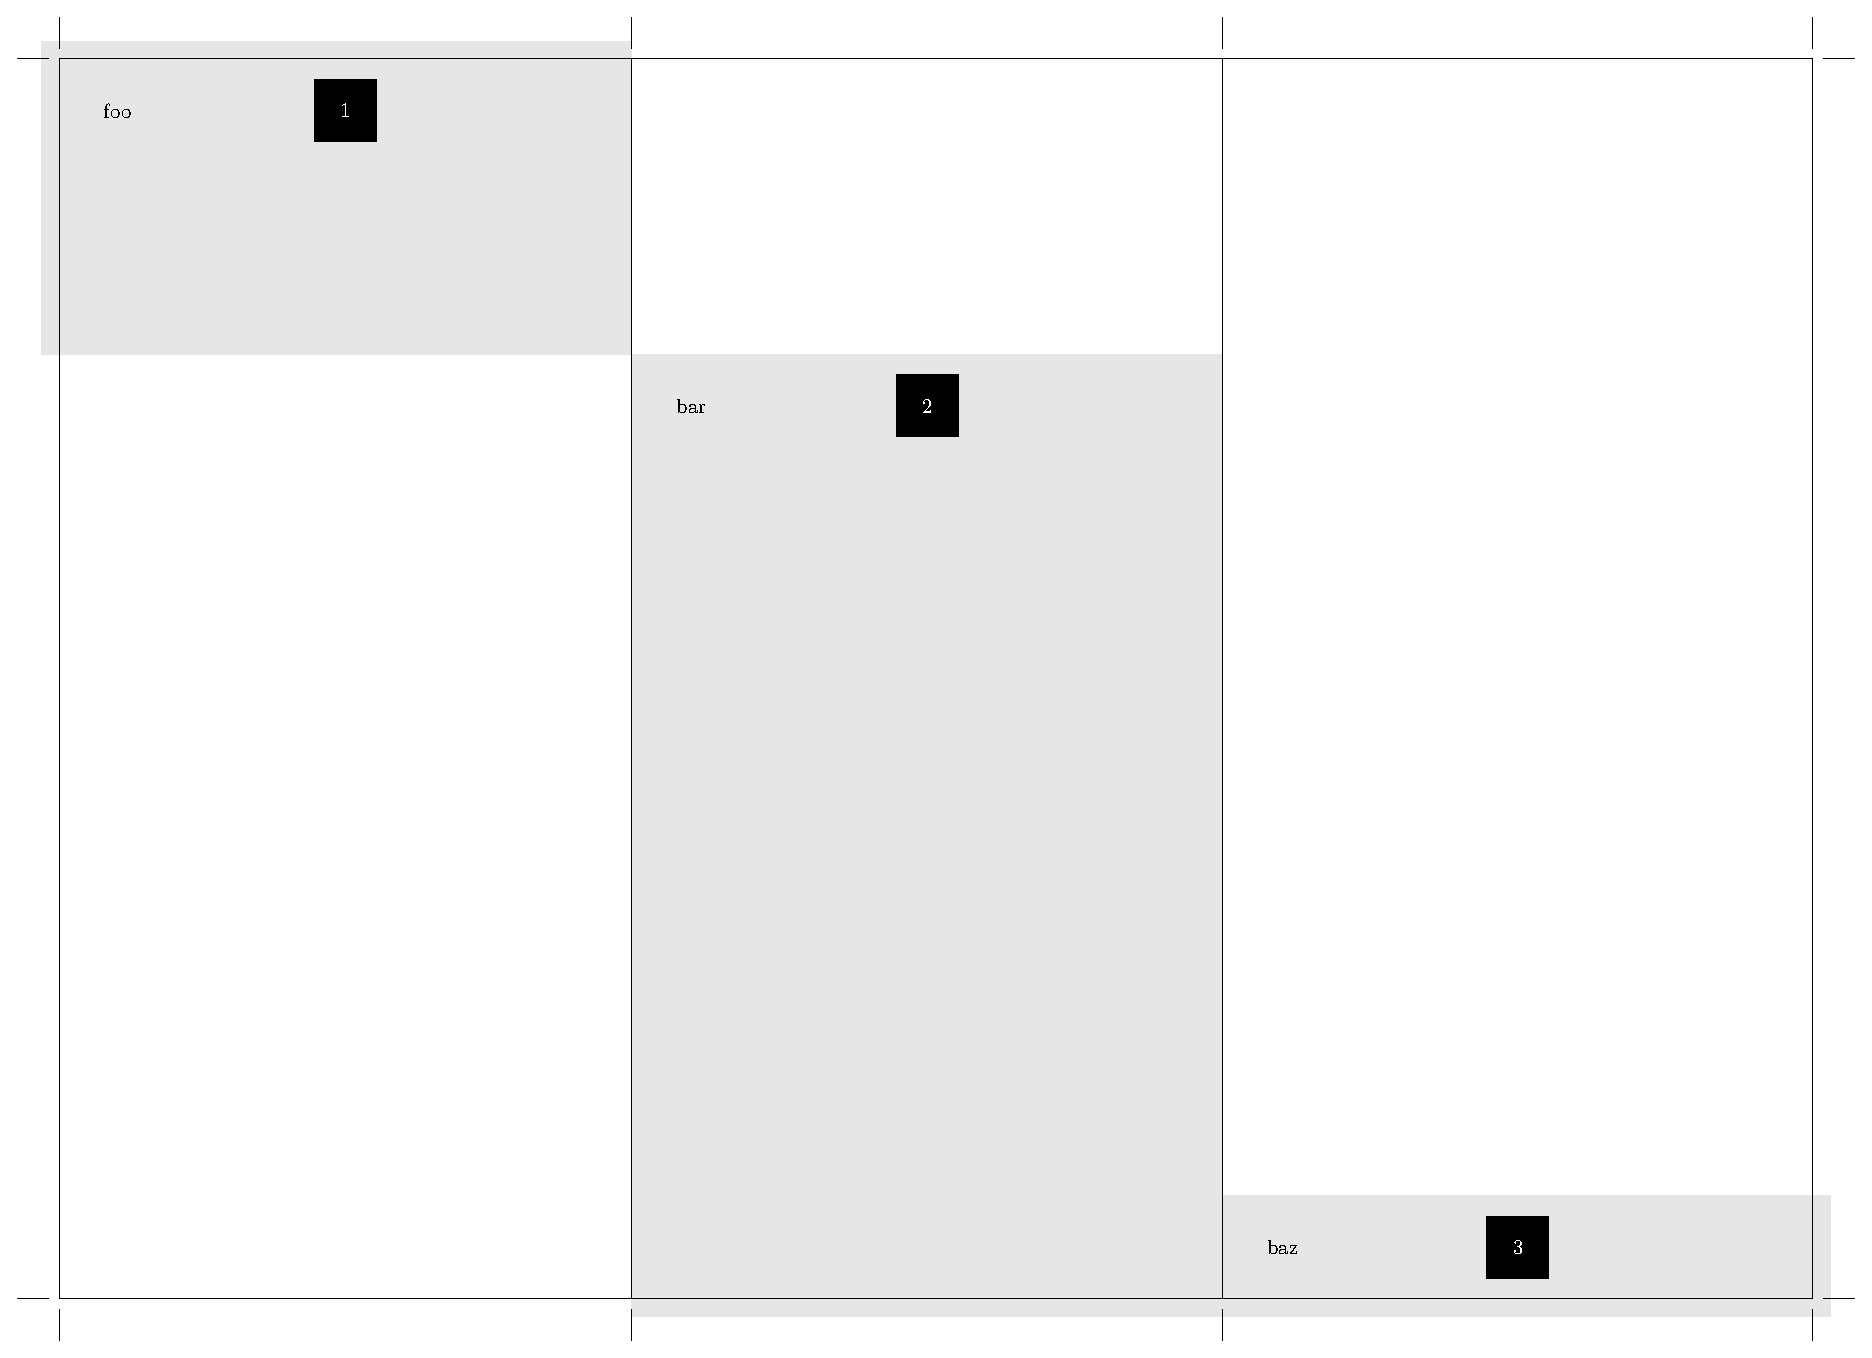
\includegraphics[width=\linewidth]{doc/layout.pdf}}
\end{tcolorbox}

\begin{codeexample}
\documentclass[
  prepress,
  show frames,
  show ids
]{leporello}

\leporellosetstyle[box]{align bottom}{
  align parent={l,b},
  align self={l,b}
}

\begin{leporellocolumn}{example-a}
\begin{leporellobox}[
  background color=black!10,
  height=50mm,
  bleed={l,t}
]
foo
\end{leporellobox}
\end{leporellocolumn}

\begin{leporellocolumn}{example-b}
\begin{leporellobox}[
  background color=black!10,
  offset={0mm,50mm},
  stretch,
  bleed={b}
]
bar
\end{leporellobox}
\end{leporellocolumn}

\begin{leporellocolumn}{example-c}
\begin{leporellobox}[
  background color=black!10,
  align bottom,
  bleed={r,b}
]
baz
\end{leporellobox}
\end{leporellocolumn}

\begin{document}

\leporellotypesetcolumns{
  example-a,
  example-b,
  example-c
}

\end{document}
\end{codeexample}

The example shows the use of the \macro{prepress} key that adds cropmarks to the layout. It also shows how the \macro{show frames} key adds frames around the columns. Finally, the \macro{show box} key adds the box IDs to the boxes.

The default layout has three pages which are shown here. Three columns named \macro{example-a}, \macro{example-b} and \macro{example-c} are defined and contain one box each. A custom style is defined to combine the two keys needed to bottom-align the third box. A fixed height is set to for the first box and the second box has and offset and its height stretched to the bottom of the column. Bleed is added to the relevant edges of the three columns.

% =====

\section{L3 commands}

\begin{macrodef}
|\l_leporello_layout_width_dim|
|\l_leporello_layout_height_dim|
\end{macrodef}
These variables hold the width and height of the layout which is the width and the height of the final printed matter without info area.

\begin{macrodef}
|\l_leporello_paper_width_dim|
|\l_leporello_paper_height_dim|
\end{macrodef}
These variables hold the width and height of the paper including info area.

\begin{macrodef}
|\l_leporello_bleed_dim|
|\l_leporello_info_area_dim|
\end{macrodef}
These variables hold the size of the bleed and the info area.

\begin{macrodef}
|\l_leporello_columns_clist|
\end{macrodef}
This variable holds the list of dimensions that represent the widths of the columns in the layout.

\begin{macrodef}
|\l_leporello_column_count_int|
\end{macrodef}
This variable holds the number of columns in the layout. It is calculated from the list of dimensions given to the \macro{global/columns} key.

\begin{macrodef}
|\l_leporello_prepress_bool|
|\l_leporello_show_frames_bool|
|\l_leporello_show_id_bool|
|\l_leporello_auto_typeset_bool|
\end{macrodef}
{\raggedright These variables hold the relevant values of the \macro{global/prepress}, \macro{global/show frames}, \macro{global/show id} and \macro{global/auto typeset} keys. \par}

\begin{macrodef}
|\l_leporello_typeset_reverse_layout_bool|
|\l_leporello_typeset_reverse_order_bool|
|\l_leporello_typeset_reverse_pagination_bool|
|\l_leporello_typeset_continuous_pagination_bool|
\end{macrodef}
{\raggedright These variables hold the relevant values of the \macro{typeset/reverse layout}, \macro{typeset/reverse order}, \macro{typeset/reverse pagination} and \macro{typeset/continuous pagination} keys. \par}

\begin{macrodef}
|\l_leporello_layout_vertical_ltr_bool|
|\l_leporello_layout_vertical_rtl_bool|
\end{macrodef}
These variables are set to true if the current layout is set to vertical and left-to-right or to vertical and right-to-left.

\begin{macrodef}
|\l_leporello_current_page_int|
|\l_leporello_current_column_int|
|\l_leporello_current_box_int|
\end{macrodef}
These variables hold the ID of the current page, the current column and the current box as integer respectively.

\begin{macrodef}
|\l_leporello_current_column_str|
\end{macrodef}
This variable holds the name of the current column.

\begin{macrodef}
|\l_leporello_image_width_dim|
|\l_leporello_image_height_dim|
|\l_leporello_image_clip_width_dim|
|\l_leporello_image_clip_height_dim|
|\l_leporello_image_scale_fp|
|\l_leporello_image_fill_bleed_bool|
\end{macrodef}
{\raggedright These variables hold the relevant values of the \macro{image/width}, \macro{image/height}, \macro{image/clip width}, \macro{image/clip height},  \macro{image/scale} and \macro{image/fill bleed} keys. \par}

\begin{macrodef}
|\g_leporello_notes_int|
\end{macrodef}
This variable holds the current counter for notes.

\begin{macrodef}
|\l_leporello_notes_list_style_str|
\end{macrodef}
This variable holds the name of the environment of the notes list. It can be changed via the key \macro{notes/list style}.

\begin{macrodef}
|\leporello_draw_absolute:nn| {<tuple of dimensions>} {<code>}
\end{macrodef}
This command typesets the code consisting of commands that are placed between \macro{\draw_begin:} and \macro{\draw_end:} by shifting it according to the offset given in the first argument. It sets the bounding box of the drawing to zero and appends a page break.

\begin{macrodef}
|\leporello_typeset_image:nn| {<key-value list>} {<file>}
\end{macrodef}
This command typesets the image from the relevant file using the options set via \macro{image/} keys.

\begin{macrodef}
|\leporello_typeset_columns:nn| {<key-value list>} {<list of strings>}
|\leporello_typeset_columns:nV| {<key-value list>} <clist varliable>
\end{macrodef}
This command is the equivalent of the user-level command \macro{\leporellotypesetcolumns}. It takes as first argument options set via \macro{typeset/} keys and as second argument a list of strings consisting of the names of the columns to be typeset.

\begin{macrodef}
|\leporello_fp_tuple_use_i:n| {<fp tuple>}
|\leporello_fp_tuple_use_i:e| {<fp tuple>}
|\leporello_fp_tuple_use_ii:n| {<fp tuple>}
|\leporello_fp_tuple_use_ii:e| {<fp tuple>}
\end{macrodef}
These commands extract the first or the second item of a floating point tuple.

\begin{macrodef}
|\leporello_note_mark:n| {<integer>}
\end{macrodef}
This command expects as argument the value of the current note counter as integer and typesets a corresponding mark. It can be changed via the key \macro{notes/mark cmd}. The default defintion is as follows:

\begin{codeexample}
\cs_new:Npn \leporello_note_mark:n #1 {
  \leporello_text_superscript:n { \int_use:N #1 }
}
\end{codeexample}

\noindent The following commands have been defined for consistency of the syntax.

\begin{macrodef}
|\leporello_ltlayout_paperwidth_set:n| {<dimension>}
|\leporello_ltlayout_paperheight_set:n| {<dimension>}
|\leporello_ltlayout_textwidth_set:n| {<dimension>}
|\leporello_ltlayout_textheight_set:n| {<dimension>}
|\leporello_ltlayout_topmargin_set:n| {<dimension>}
|\leporello_ltlayout_oddsidemargin_set:n| {<dimension>}
|\leporello_ltlayout_evensidemargin_set:n| {<dimension>}
|\leporello_ltlayout_hoffset_set:n| {<dimension>}
|\leporello_ltlayout_voffset_set:n| {<dimension>}
|\leporello_ltlayout_headheight_set:n| {<dimension>}
|\leporello_ltlayout_headsep_set:n| {<dimension>}
|\leporello_ltlayout_footskip_set:n| {<dimension>}
|\leporello_ltlayout_marginparwidth_set:n| {<dimension>}
|\leporello_ltlayout_marginparsep_set:n| {<dimension>}
|\leporello_ltlayout_marginparpush_set:n| {<dimension>}
\end{macrodef}
These commands set the relevant LaTeX dimension to the argument given. To give an example, \macro{\leporello_ltlayout_paperwidth_set:n {297mm}} sets \macro{\paperwidth} to 297mm.

\begin{macrodef}
|\leporello_pagestyle_set:n| {<string>}
\end{macrodef}
The command \macro{\leporello_pagestyle_gset:n {#1}} is a wrapper for \macro{\pagestyle{#1}} to set the page style.

\begin{macrodef}
|\leporello_page_gset:n| {<integer>}
\end{macrodef}
The command \macro{\leporello_page_gset:n {#1}} is a wrapper for \macro{\setcounter{page}{#1}} to set the current page number.

\begin{macrodef}
|\leporello_text_superscript:n| {<token list>}
\end{macrodef}
{\raggedright The command \macro{\leporello_text_superscript:n {#1}} is a wrapper for \macro{\textsuperscript{#1}}. \par}

\begin{macrodef}
|\leoprello_graphics_use:nn| {<key-value list>} {<file>}
\end{macrodef}
{\raggedright The command \macro{\leoprello_graphics_use:nn {#1} {#2}} is a wrapper for \macro{\includegraphics[#1]{#2}}. \par}

% =====

\printchanges

\end{document}

%% End of file `leporello-doc.tex`.